\documentclass[../main.tex]{subfiles}

\begin{document}

\section{Lecture \#1: Introduction to GMs}
\begin{itemize}
  \item Graphical model is a method of modeling a probability distribution for reasoning under uncertainty
  \item Three important questions: 1) representation, 2) inference, and 3) learning
  \item Benefits of GMs:
  \begin{itemize}
    \item 1) reduces the number of parameters required to describe the joint distribution of a set of random variables
    \item a full joint distribution would require $2^{n - 1}$ where n is the number of variables parameters
    \item 2) data integration, each term becomes self-contained and we can estimate terms with only the relevant data points
    \item problem of joint estimation n be modularized
    \item 3) generic method of representing knowledge and making inferences
    \item inject domain knowledge through priors
  \end{itemize}
  \item Bayes Net is represented by a DAG
  \item Each node in a Bayes net has a Markov blanket = its parents, children, and children's parents
  \item Every node is conditionally independent of nodes outside its Markov blanket
  \item Markov Random Field uses an undirected graph and every node is conditionally independent of all nodes other than its immediate neighbors
  \item \href{https://sailinglab.github.io/pgm-spring-2019/notes/lecture-01/}{Notes 2019}
  \item \href{https://www.cs.cmu.edu/~epxing/Class/10708-20/lectures.html}{Notes 2020}
\end{itemize}

\section{Lecture \#2: Bayesian Networks}
\begin{itemize}
  \item \textbf{Evaluation:} how likely is the sequence of observations?
  \item \textbf{Decoding:} what portion of the sequence was generated with the fair die, and what portion with the loaded die?
  \item \textbf{Learning:} how "loaded" is the loaded die?
  \item We can model the casino problem using a Hidden Markov Model (HMM)
  \item The past is conditionally independent of the future given the present (Markov property)
  \item
  \item \href{https://sailinglab.github.io/pgm-spring-2019/notes/lecture-02/}{Notes}
\end{itemize}

\section{Lecture \#3: Parameter Estimation}
\begin{itemize}
  \item GM learning can be split into: structural learning and parameter learning
  \item Learning parameters for BN that has known, fixed structure and completely observable
  \item We have a dataset of $N$ iid examples $D = \{x_{1}, \dotsc, x_{N}\}$
  \item \textit{Exponential family} is a parametric set of probability distributions that characterize many distributions like Bernoulii, Multinomial, Gaussian, Poisson, and Gamma
  \begin{align*}
    p(x|\eta) &= h(x)\text{exp}[\eta^{T}T(x) - A(\eta)] \\
              &= \frac{1}{Z(\eta)}h(x) \text{exp}[\eta^{T}T(x)]
  \end{align*}
  \begin{conditions}
    A(\eta) & log normalizer \\
    T(x) & sufficient statistic \\
    \eta & canonical parameter
  \end{conditions}
  \item Easy to compute $q-th$ central moments of exponential family distributions by taking $q-th$ derivative of the log normalizer $A(\eta)$
  \item 1-to-1 relationship between canonical and moment parameters, $\eta = \psi(\mu)$
\end{itemize}

\subsection{Generalized Linear Models (GLIMs)}
  \begin{itemize}
    \item Input enters the model via a linear combination $\xi = \theta^{T}x$
    \item $\mu$ is a function of $\xi: f(\xi)$
    \item Output $y$ is characterized by an exponential family distribution $p$
    \item $E_{p}(y) = \mu = f(\theta^{T}x)$ is a GLIM
    \item Examples of GLIM include linear regression and logistic regression
    \item Other examples: MRFs, Restricted Boltzmann Machines, CRFs
    \item MLE for learning GLIMs (?)
    \item MLE of a normal distribution, we take the log-likelihood of $l(\mu)$ and take the derivative wrt to $\mu$, set equal to 0 and solve for $\mu$, we get that $\mu_{MLE} = \frac{1}{n} \sum_{i=1}^{n} x_{i}$
    \item In GMM, each cluster corresponds to a Gaussian distribution and there are $k$ clusters
    \item Parameters are $\theta = \{\mu_{1}, \dotsc, \mu_{K}, \sigma_{1}, \dotsc, \sigma_{K}, \pi_{1}, \dotsc, \pi_{K}\}$ where $\pi_{k}$ is the mixture proportion representing probability that $X_{i}$ belongs to the $k$-th mixture component
    \item MLE for GMM is different because we can't analytically solve for $\mu$ because of summation. Would be easy if we new the latent variables $Z_{i}$ or cluster assignments
    \item EM is sensitive to initialization of parameters
    \item EM is used to find ML estimates for models with latent variables
    \item E-step use current value of parameters to find posterior distribution of latent variable: $P(Z|X, \theta^{0}$
    \item M-step determine new parameters $\hat{\theta}$
    \item \href{https://stephens999.github.io/fiveMinuteStats/intro_to_em.html}{Nice tutorial on EM}
  \end{itemize}

\subsection{Parameter Estimation for Partially Observed GMs}
  \begin{itemize}
    \item Often some RVs for GMs may be unobserved, some are not physically measurable, some are not observed because of faulty sensors
    \item Want to estimate parameters of a GMM given partially observed data using the EM Algorithm
    \item EM alternates between 1) computing cluster assignments at time t using the means at time t and 2) using the cluster assignments at time t to recompute mean for next iteration
  \end{itemize}

\section{Lecture \#6: Case studies: HMM and CRF}

\section{Lecture \#7: Variation Inference 1}
\begin{itemize}
  \item VI converts inference into optimization, approximate desired solution by relaxing intractable optimization problem
  \item e.g. linear systems of equation that is too large to invert
  \item There is some probability distribution $P$ that we can't perform inference on, try to approximiate $P$ with another distribution $Q$
  \item Requires some way to measure distance between $P$ and $Q$ (usually KL)
  \item
\end{itemize}

\section{Lecture \#9: Sampling 1}
\begin{itemize}
  \item Inference method for an arbitrary distribution
  \item Instead of manipulating $P(X)$, we estimate it using samples from the distribution
  \item Drawback of naive sampling is that for large models, it is difficult to get estimates for rare events
  \item Rejection sampling: sample from a simpler distribution $Q(x)$ and accept sample with probability
  \item If $Q(x)$ is not chosen well, we will get a lot of rejectd samples
  \begin{itemize}
    \item Sample $x_{0}$ from $q_{x}$
    \item Sample a number $u_{0}$ from uniform distribution over $[0, kq(x_{0})]$ where $k$ is a constant such that $kq(x) \geq \tilde{p}(x)$
    \item Reject if $u_{0} > \tilde{p}(x_{0})$
  \end{itemize}
  \item Importance sampling:
  \begin{itemize}
    \item
  \end{itemize}
\end{itemize}
\subsection{Markov Chain Monte Carlo (MCMC)}
\begin{itemize}
  \item Metropolis-Hastings Algorithm
  \begin{itemize}
    \item MH works by simulating a Markov Chain whose stationary distribution is $\pi$
    \item Idea is that instead of using a fixed $Q(x)$ like likelihood weighting, we use an adaptive proposal $Q(x'|x)$
    \begin{figure}[h]
      \caption{Adaptive Proposal}
      \centering
      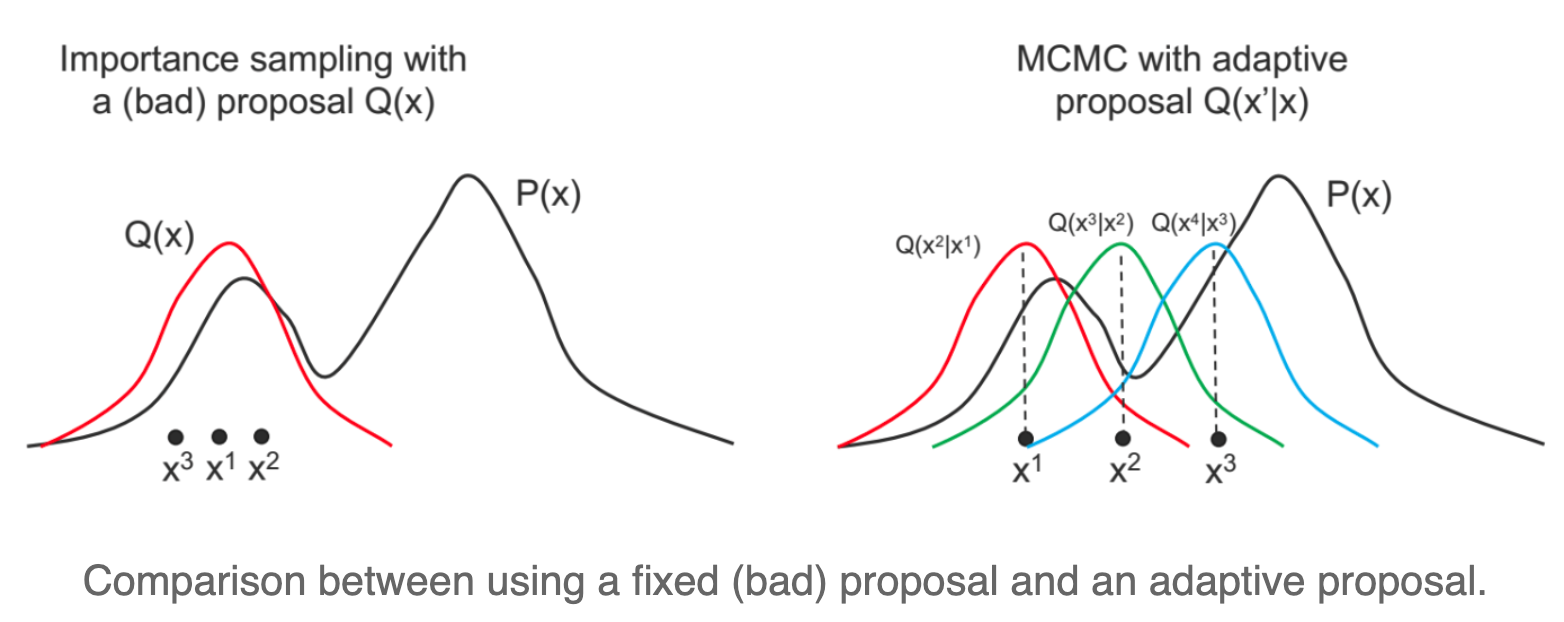
\includegraphics[width=\textwidth]{../imgs/adaptive_proposal.png}
    \end{figure}
    \item MH has a "burn-in" period where an initial number of samples are thrown away because they are not from the true distribution
  \end{itemize}
  \item The user needs to provide a "transition kernel", $Q$. $Q$ is often a continuous distribution. Random walk kernel: $Q(y|x) = \frac{1}{\sqrt{2\pi}}\text{exp}^{-0.5(y-x)^{2}}$
  \item \href{https://stephens999.github.io/fiveMinuteStats/MH_intro.html}{MH tutorial}
  \item Gibbs Sampling
  \item Suppose there is some $p(x,y)$ that is difficult to sample from directly
  \item $p(x|y)$ and $p(y|x)$, the conditional distributions are easier to sample from
  \item Also has a "burn-in" period
  \item GS is a special case of MH
  \item Practical aspects:
  \begin{itemize}
    \item Evaluate $Q(x'|x)$: acceptance rate, autocorrelation function
    \item When to stop burn-in: plot the log-likelihood v.s. time
  \end{itemize}
\end{itemize}
\begin{algorithm}[H]
    \SetAlgoLined
    Initialize $X_{1} = x_{1}$\;
    \For{t = 1,2,...} {
      Sample $y$ from $Q(y|x_{t})$\;
      $A = min(1, \frac{\pi(y)Q(x_{t}|y)}{\pi(x_{t}Q(y|x_{t}))})$, $A$ is the "acceptance probability"\;
      If Q is symmetric, the formula for $A = min(1, \frac{\pi(y)}{\pi(x_{t})})$\;
      Accept $y$ with probability $A$ and set $x_{t+1} = y$
    }
    \caption{MH algorithm}
\end{algorithm}
\begin{algorithm}[H]
    \SetAlgoLined
    Set $x$ and $y$ to some initial starting values: $(x_{0}, y_{0})$\;
    Sample $x|y$, $x_{1} \sim p(x|y_{0})$ and then sample $y|x$, $y_{1} \sim p(y|x_{1})$\;
    Repeat\;
    \caption{Gibbs Sampling}
\end{algorithm}

\subsection{Important probability distributions}
  \begin{itemize}
    \item Multinomial
    \begin{itemize}
      \item $K$-outcome multinomial distribution
      \item generalization of the Bernoulli distribution
      \item models probability of counts for a k-sided die rolled n times
      \item $k = 2$ and $n = 1$, the multinomial distribution is the Bernoulli
      \item $k = 2$ and $n > 1$, this is the binomial distribution
      \item $k > 2$ and $n = 1$, this is the categorical distribution
    \end{itemize}
    \begin{align*}
      p(x|\pi) = \pi_{1}^{x_{1}}\pi_{2}^{x_{2}} \dotsc \pi_{K}^{x_{K}}
    \end{align*}
    \item Bernoulii
    \begin{itemize}
      \item probability that flipping a coin one time will result in heads or tails
    \end{itemize}
    \item Gaussian
    \begin{itemize}
      \item k-dimensional Gaussian
      \begin{align*}
        p(x|\mu, \Sigma) &= \frac{1}{(2\pi)^{k/2}|\Sigma|^{\frac{1}{2}}}\text{exp}\{\frac{1}{2}(x-\mu)^{T}\Sigma^{-1}(x-\mu)\} \\
        &= \frac{1}{(2\pi)^{\frac{k}{2}}}\text{exp}\{-\frac{1}{2}\text{Tr}(\Sigma^{-1}xx^{T} + \mu^{T}\Sigma^{-1}x - \frac{1}{2}\mu^{T}\Sigma^{-1}\mu - log|\Sigma|\}
      \end{align*}
    \end{itemize}
    \item Poisson
    \begin{itemize}
      \item used for modeling the number of times an event occurs in an interval of time or space
      \item $\text{Pois}(\lambda) = \frac{\lambda^{k}e^{-\lambda}}{k!}$
    \end{itemize}
    \item Gamma
  \end{itemize}

\subsection{Markov Chain Concepts}
  \begin{itemize}
    \item Markov Chain is a sequence of RVs with the Markov Property: $P(x^{(n)} = x | x^{(1)}, \dotsc, x^{(n-1)}) = P(x^{(n)} = x | x^{(n-1)})$
    \item Transitions
    \item \textbf{Stationary distributions:} if it does not change under transition kernel, $\pi(x') = \sum_{x} \pi(x)T(x'|x)$
    \item Intuition: in the long run, no matter where the starting state was, the proportion of time the chain spends in state $j$ is approximately $\psi_{j}$ for all $j$, i.e. $\psi P = \psi$
    \item \textbf{Irreducible}: you can get from any state $x$ to another other state $x'$ with probability $> 0$ in a finite number of steps
    \item Aperiodic: you can return to any state $x$ at any time
    \item \textbf{Ergodic}: irreducible and aperiodic
    \item Erogdicity implies you can reach the stationary distribution no matter the initial distribution
    \item \textbf{Reversible}: there exists a distribution $\pi(x)$ such that $\pi(x')T(x|x') = \pi(x)T(x'|x)$
    \item Reversible MCs \textbf{always} have a stationary distribution
  \end{itemize}

\end{document}